\section{Torsional Resonance Model}\label{sec:trModel}
A system with TR typically consists of three main items;
An actuator, or motor, with a given inertia, $J_a$, and damping, $B_a$, associated with it.
An inertial load, $J_L$, with a given damping, $B_L$, associated with it.
A coupler between the actuator and the load with a spring constant, $K_c$, and a damping, $B_c$, associated with it.


It is assumed that the inertia of the coupler is included in the inertia of the actuator and the load. The physical diagram of the system with TR can be found in Fig.\ref{fig:couple}. In order to find the transfer function for this system, where $T_{in}$ is the torque input and the actuator angle $\theta_a$ is the output, the physical diagram is then converted into a mechanical network, see Fig.~\ref{fig:mech}, so the system's dynamics can be written as

\begin{figure}[h]
  \centering
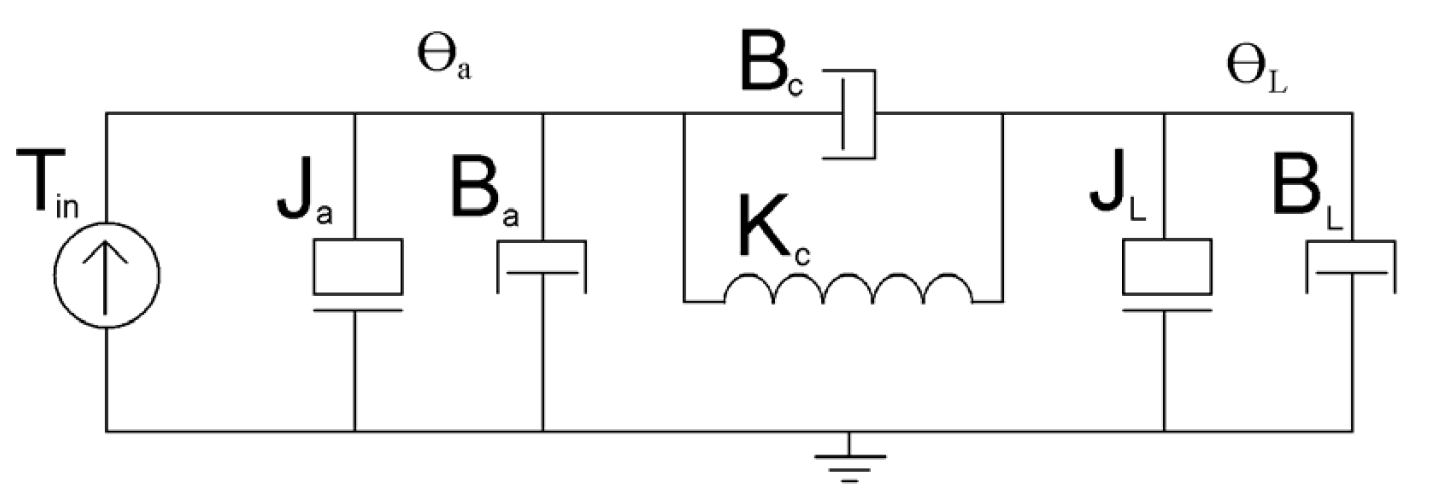
\includegraphics[width=1.0\columnwidth]{./pix/mech.png}
  \caption{Mechanical schematic drawling of system with TR}
  \label{fig:mech}
\end{figure}

\begin{equation}
%T(t) = J_a\ddot{\theta_a}+\left( B_a+B_c \right) \dot{\theta_a}=K_c\theta_a-\left(K_c\theta_L+B_c\dot{\theta_L}\right)
T(t) = J_a\ddot{\theta_a}+(B_a+B_c ) \dot{\theta_a}=K_c\theta_a-(K_c\theta_L+B_c\dot{\theta_L})
\end{equation}

and



\begin{equation}\label{eq:thetaLthetaa}
\frac{\theta_L}{\theta_a} = \frac{K_c+sB_c}{s^2+J_L+sB_L+K_c+sB_c}
\end{equation}

is the relationship between $\theta_L$ and $\theta_a$ as shown as the ratio of $\frac{\theta_L}{\theta_a}$. Note that $\theta_a$ contains up to and including first order terms and $\theta_L$ includes up to and including second order terms.  The relationship between $\theta_a$ and torque, $T$, is represented as


%\begin{equation}
%T(s) = \left( (s^2J_a+sB_a+K_c+sB_c)- \frac{(K_c+sB_c)(K_c+sB_c)}{s^2J_L + sB_L + K_c +sB_c}\right) \theta_a
%\end{equation}


\begin{equation}\label{eq:tf}
\frac{\theta_a(s)}{T(s)} = \frac{  \frac{1}{J_aJ_L}\left(s^2J_L+K_c + sB_c\right)  }{s^2 \left( s^2+B_c\frac{J_a+J_L}{J_aJ_L} s + K_c \frac{J_a+J_L}{J_aJ_L} \right)}
%\frac{\theta_a(s)}{T(s)} = \frac{\frac{1}{J_aJ_L}(s^2J_L+s(B_L+B_c)+Kc)}{s^4 + K_1\frac{s^3}{J_aJ_L} + K_2\frac{s^2}{J_aJ_L} + K_3\frac{s}{J_aJ_L}}
\end{equation}

In this system $B_a << B_L$ therefore $B_a$ is assumed to be zero.









The poles of a system with TR (\ref{eq:tf}) consists of a double pole at the origin and complex conjugate (CC) poles.  The CC poles are in the left half plane (LHP) as long as the following inequality is satisfied.

\begin{equation}
4K_c > B_c^2 \left( \frac{J_c+J_L}{J_aJ_L} \right)
\end{equation}


\noindent The system can represented in state space as

\begin{equation}\label{eq:ssTR}
\begin{array}{lllllll}

\left[
\begin{array}{l}
\ddot{\theta_a} 	\\ 
\dot{\theta_a}		\\
\ddot{\theta_L}	\\
\dot{\theta_L}
\end{array}
\right]



&


=

&

A

&

\left[
\begin{array}{l}
\dot{\theta_a} 	\\ 
\theta_a		\\
\dot{\theta_L}	\\
\theta_L
\end{array}
\right]

&

+

&

B

&

T(t)


\end{array}
\end{equation}


where


\begin{equation}
\begin{array}{lll}
A
&
=
&

\left[
\begin{array}{cccc}
\frac{-(B_a+B_c)}{J_a}   	& \frac{-K_c}{J_a}   	& \frac{B_c}{J_a}   		&	\frac{K_c}{J_a} \\
1 					& 0				& 0					&	0			\\
\frac{B_c}{J_L}			& \frac{K_c}{J_L}	& \frac{-(B_c+B_L)}{J_L}	& 	\frac{-K_c}{J_L} \\
0					& 0				& 0					&	1		
\end{array}

\right]


\end{array}
\end{equation}



\begin{equation}
\begin{array}{lllrrr}
B

&

=

&

\left[
\begin{array}{r}
J^{-1}_a 	\\ 
0		\\
0	\\
0
\end{array}
\right]
,
&
C
&
=
&
\left[
\begin{array}{cccc}
0 	&	1	&	0	&	0
\end{array}
\right]




\end{array}
\end{equation}


\noindent standard techniques show that the system is fully controllable and with the angular position $\theta_a$ being the only output is also fully observable.  The controllability and observability matrix are both full rank.



%A system exhibiting TR has a non-zero spring constant in the coupler $K_c$. 
The resonance and anti-resonance frequencies, $\omega_r$ and $\omega_{ar}$, are defined by the inertial load of coupled system as well as the spring constant of the coupler $K_c$, Eq.\ref{eq:res}\cite{chmielewski}.
Fig.~\ref{fig:trBode} shows the frequency response of a system that is:
\begin{itemize}
\item exhibiting TR
\item not exhibiting TR with a total inertial load of $J_a$
\item not exhibiting TR with a total inertial load of $J_a+J_L$.  
\end{itemize}
The dominant load before resonance is the total inertial load ($J_a+J_L$) where after resonance it is only the actuator's inertia.  The resonance $\omega_r$ and anti-resonance $\omega_{ar}$ can be calculated by


\begin{equation}\label{eq:res}
\begin{array}{cc}

\omega_{ar} = \left(\frac{K_c}{J_L}\right)^\frac{1}{2}

&

\omega_{r} = \left(\frac{K_c}{\frac{J_aJ_L}{J_a+J_L}}\right)^\frac{1}{2}
\end{array}
\end{equation}

\noindent and the gain separation when going from an acting load of $J_L+J_a$ to $J_a$, as seen in Fig.~\ref{fig:trBode}, is calculated by Chmielewski et. al.\cite{chmielewski} and is

\begin{equation}\label{eq:deltaDB}
\Delta dB = 40\mbox{log}_{10}\left(\frac{\omega_r}{\omega_{ar}}\right)
\end{equation}


\begin{figure}[ht]
  \centering
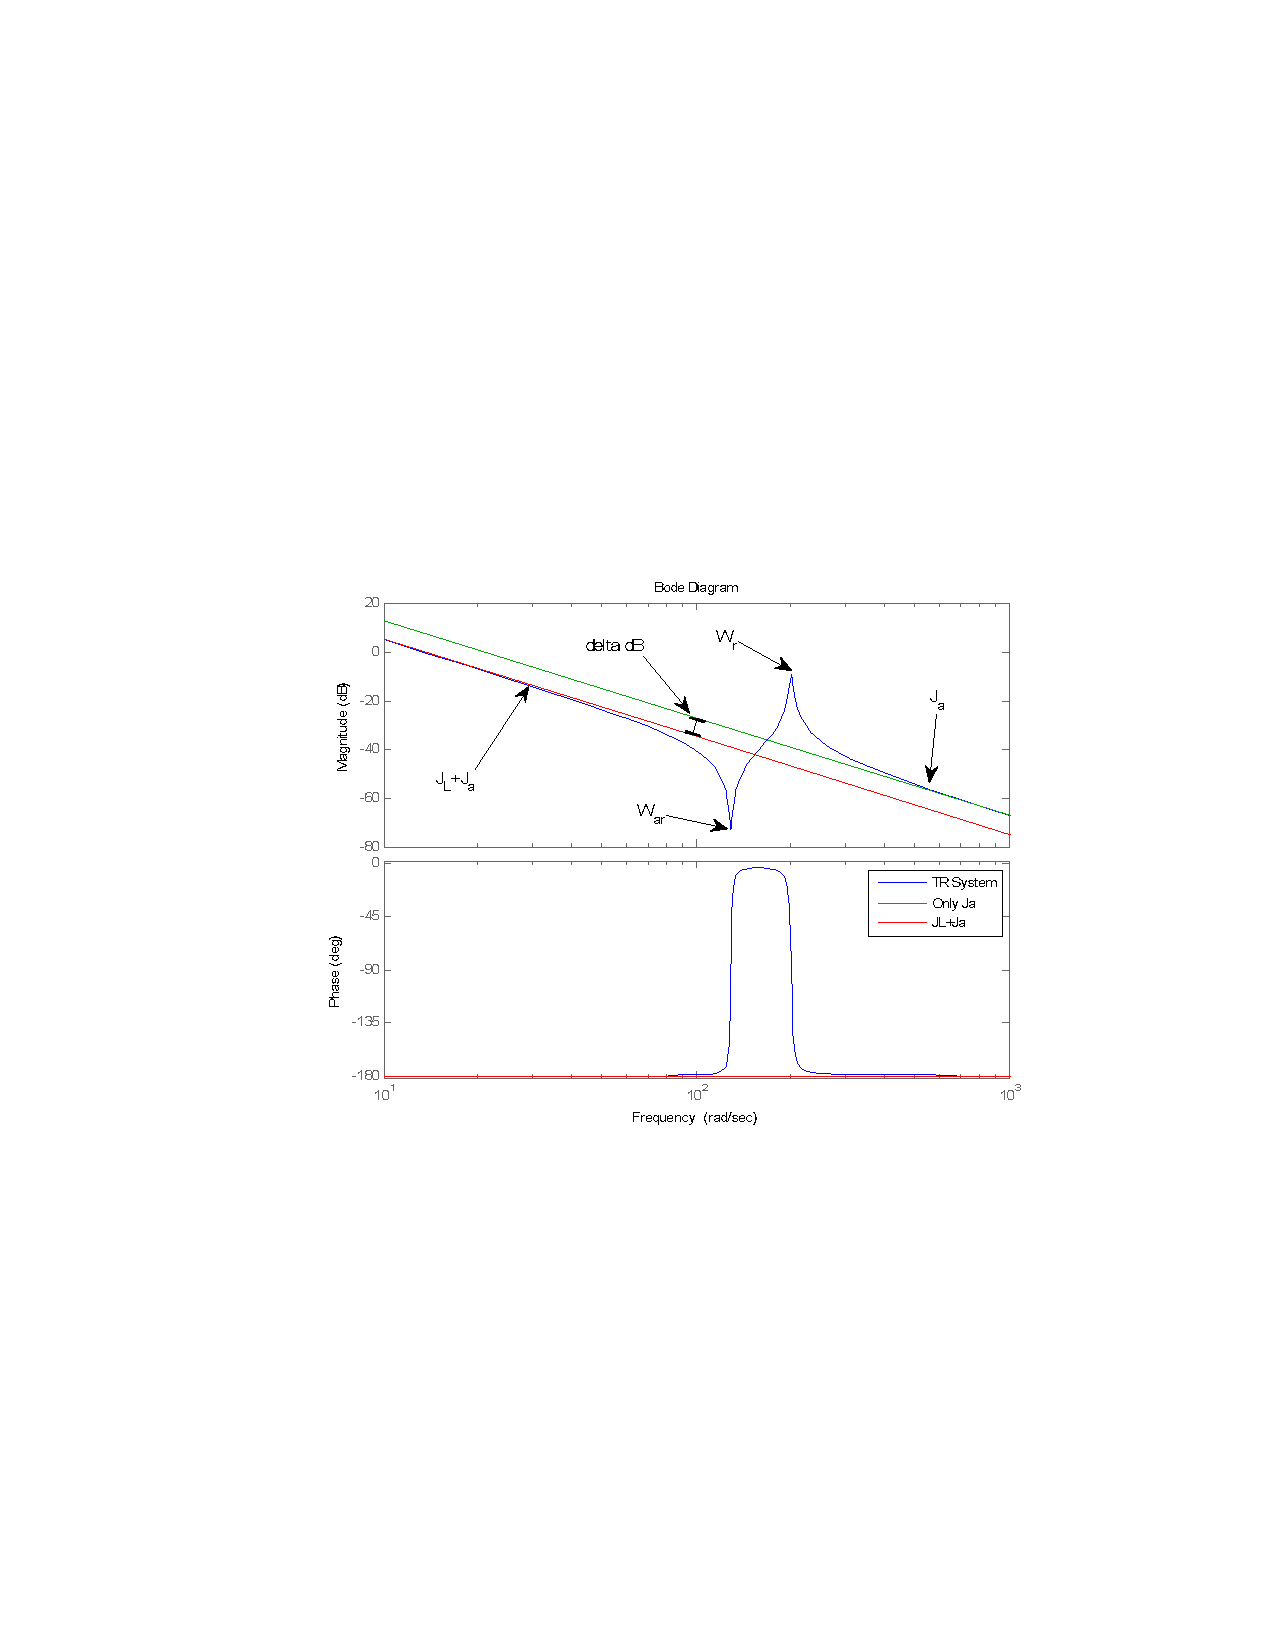
\includegraphics[width=1.0\columnwidth]{./pix/bode.pdf}
  \caption{Frequency Response Plot of System with TR (from Eq. \ref{eq:ssTR}), System with no TR with
inertial load of $J_a$, and System with no TR and inertial load of $J_a+J_L$}
  \label{fig:trBode}
\end{figure}

